%! Author = Сергей
%! Date = 27.02.2023

% Preamble
\documentclass[tikz, margin=3mm]{standalone}

% Packages
\usepackage[utf8]{inputenc}
\usetikzlibrary{shapes.geometric, arrows}

% Tikz styles
\tikzstyle{startstop} = [
    rectangle, rounded corners,
    minimum width=3cm, minimum height = 1cm,
    text centered,
    draw=black, fill=red!30
]
\tikzstyle{io} = [
    trapezium, trapezium left angle=70, trapezium right angle=110,
    minimum width=3cm, minimum height = 1cm,
    text centered,
    draw=black, fill=blue!30
]
\tikzstyle{process} = [
    rectangle,
    minimum width=3cm, minimum height = 1cm,
    text centered, text width=3cm,
    draw=black, fill=orange!30
]
\tikzstyle{decision} = [
    diamond,
    minimum width=3cm, minimum height = 1cm,
    text centered,
    draw=black, fill=green!30]
\tikzstyle{arrow} = [thick,->,>=stealth]

% Document
\begin{document}
    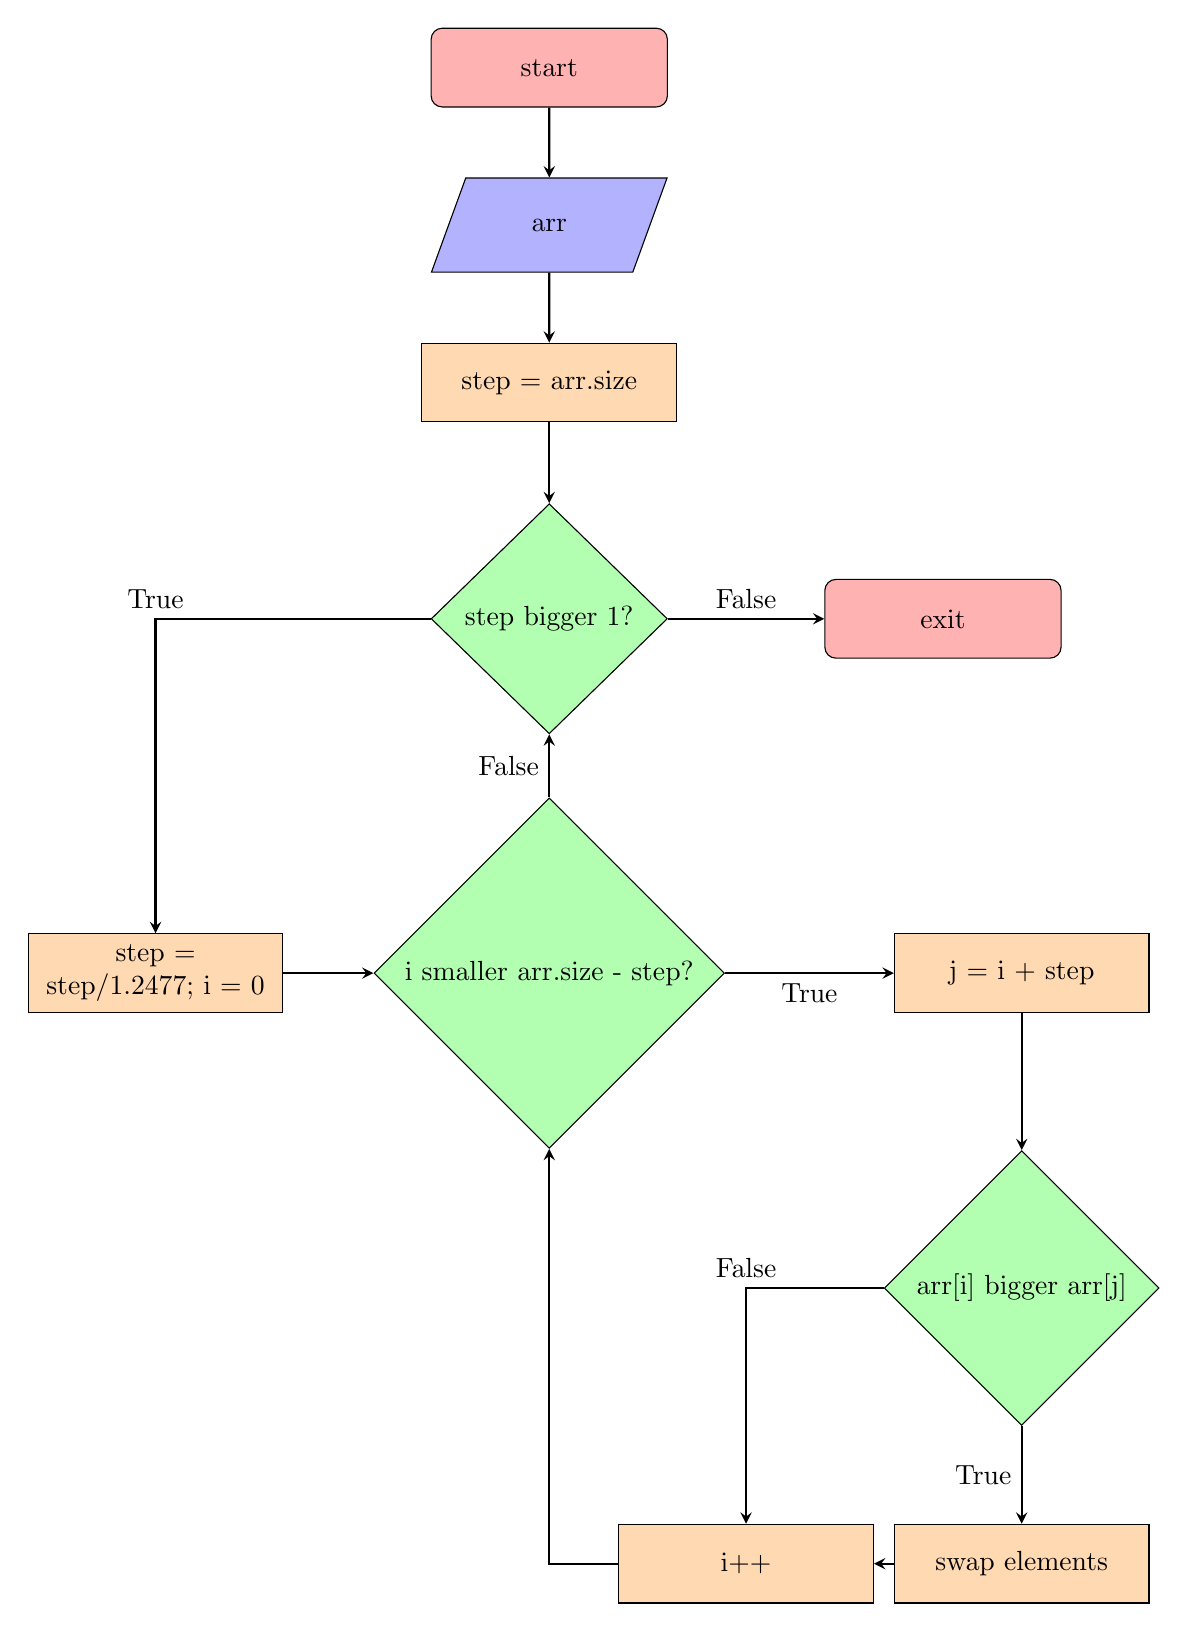
\begin{tikzpicture}[node distance=2cm]
        % Draw blocks
        \node (start) [startstop, yshift=10cm] {start};
        \node (input) [io, below of=start] {arr};
        \node (defstep) [process, below of=input] {step = arr.size};
        \node (d1) [decision, below of=defstep, yshift=-1cm] {step bigger 1?};
        \node (step1247) [process, left of=d1, xshift=-3cm, yshift=-4.5cm] {step = step/1.2477; i = 0};
        \node (d2) [decision, right of=step1247, xshift=3cm] {i smaller arr.size - step?};
        \node (defj) [process, right of=d2, xshift=4cm] {j = i + step};
        \node (d3) [decision, below of=defj, yshift=-2cm] {arr[i] bigger arr[j]};
        \node (swap) [process, below of=d3, yshift=-1.5cm] {swap elements};
        \node (incr) [process, left of=swap, xshift=-1.5cm] {i++};
        \node (stop) [startstop, right of=d1, xshift=3cm] {exit};

        % Draw arrows
        \draw [arrow] (start) -- (input);
        \draw [arrow] (input) -- (defstep);
        \draw [arrow] (defstep) -- (d1);
        \draw [arrow] (d1) -| node[anchor=south] {True} (step1247);
        \draw [arrow] (d1) -- node[anchor=south] {False} (stop);
        \draw [arrow] (step1247) -- (d2);
        \draw [arrow] (d2) -- node[anchor=north] {True} (defj);
        \draw [arrow] (d2) -- node[anchor=east] {False} (d1);
        \draw [arrow] (defj) -- (d3);
        \draw [arrow] (d3) -- node[anchor=east] {True} (swap);
        \draw [arrow] (d3) -| node[anchor=south] {False} (incr);
        \draw [arrow] (swap) -- (incr);
        \draw [arrow] (incr) -| (d2);
    \end{tikzpicture}
\end{document}